\documentclass[10pt,twocolumn]{article}
\usepackage[margin=0.75in]{geometry}
\usepackage{enumitem}
\usepackage{booktabs}
\usepackage{hyperref}
\usepackage{graphicx}
\usepackage{titlesec}
\usepackage{parskip}
\usepackage{tabularx}
\usepackage{amsmath}
\usepackage{xcolor}
\usepackage{multicol}
\usepackage{caption}
\usepackage{pgfplots}
\pgfplotsset{compat=1.18}

\titlespacing*{\section}{0pt}{8pt}{4pt}
\titlespacing*{\subsection}{0pt}{6pt}{2pt}
\titleformat{\section}{\normalfont\large\bfseries}{\thesection.}{0.5em}{}
\titleformat{\subsection}{\normalfont\normalsize\bfseries}{\thesubsection}{0.5em}{}

\setlength{\columnsep}{0.25in}
\setlist{nosep,leftmargin=*}
\renewcommand{\arraystretch}{1.1}

\title{\vspace{-1.5cm}\textbf{Project 42: Terraform Smart Context MCP Server}\\[4pt]\large Progress Report -- CS 6650 Distributed Systems}
\author{
  Kalhar Pandya \and Vinal Dsouza \and Parin Shah\\[2pt]
  \small Northeastern University Vancouver\\[2pt]
  \small \url{https://github.com/KalharPandya/terraform-smart-context-mcp-42}\\
  \small Project Board: \url{https://github.com/users/KalharPandya/projects/1}
}
\date{March 29, 2026}

\begin{document}
\maketitle
\vspace{-0.5cm}

\section{Problem, Team, and Experiments}

\subsection{The Problem}

Large Language Models are increasingly used as infrastructure operators, but when an LLM queries what is \textit{actually deployed}, it faces three failures: \textbf{(1)} State is too large -- \texttt{terraform show -json} on a 75-resource project produces 4,041 lines ($\sim$33K tokens); \textbf{(2)} Every interaction starts blind with no memory of deployments; \textbf{(3)} Without structured access, agents hallucinate resource arguments and generate configs that fail against real APIs.

Code editing agents (Cursor, Claude Code) solved this for programming with structured tools. Terraform has no equivalent. Project~42 builds an MCP server that gives any AI agent structured, token-efficient access to live Terraform infrastructure -- so the agent queries exactly what it needs instead of drowning in raw state.

\textbf{Stakeholders:} DevOps teams at scale, platform engineers, any organization with 50+ Terraform resources where per-query cost matters.

\subsection{The Team}

\begin{table}[h]
\centering\small
\begin{tabularx}{\columnwidth}{lXX}
\toprule
\textbf{Member} & \textbf{Role} & \textbf{Expertise} \\
\midrule
Kalhar Pandya & Implementation, architecture & TypeScript, MCP SDK \\
Vinal Dsouza & AI-first workflow, alignment & Claude Code automations \\
Parin Shah & Protocol design, experiments & Scorer, prompt engineering \\
\bottomrule
\end{tabularx}
\end{table}

\subsection{Experiments and AI Role}

Three experiments evaluate whether purpose-built MCP tools improve LLM-infrastructure interaction. Metrics: accuracy, tokens, cost, tool calls, latency. \textit{Context Efficiency} = Total Tokens / Correct Answers.

\begin{table}[h]
\centering\small
\begin{tabularx}{\columnwidth}{lXl}
\toprule
\textbf{\#} & \textbf{Question} & \textbf{Status} \\
\midrule
1 & Do MCP tools reduce cost while maintaining accuracy? & Baseline done \\
2 & Coarse vs.\ fine-grained tool responses? & Designed \\
3 & Does the server work across 15 models? & Designed \\
\bottomrule
\end{tabularx}
\end{table}

AI plays a \textbf{dual role}: development tool (Claude Code with 7 slash commands, 5 domain skills) and experiment subject (the agent tested with/without MCP tools).

\subsection{Observability}

Experiment layer: \texttt{runner.ts} captures tokens, cost, time, tool calls per trial. MCP server (planned): structured JSON logging per tool invocation (\texttt{tool, latency\_ms, response\_size, error}). Visualization: \texttt{visualize.ts} generates Chart.js dashboard with 6 interactive charts.

\section{Project Plan and Progress}

\subsection{Timeline}

Project deadline: \textbf{April 10, 2026}. Two sprints. Tracked via GitHub Projects with 23 issues.

\textbf{Sprint 1 (Complete, Mar 28--29):} 75-resource dummy infra (\#12), 10 prompts with ground truth (\#13), experiment runner (\#14), scorer (\#15), baseline experiment -- 30 trials, \$1.73 (\#16), v1 tool set design, 5 architecture decisions (\#7--11).

\textbf{Sprint 2 (Mar 30 -- Apr 10):} DAG engine + traversal (\#17--18), purpose-built tools (\#19--20), GraphQL schema + tools (\#21--22), integration (\#23), Experiment~1 MCP arm, final report.

\begin{table}[h]
\centering\small
\begin{tabularx}{\columnwidth}{lXl}
\toprule
\textbf{Member} & \textbf{Sprint 1 (Done)} & \textbf{Sprint 2} \\
\midrule
Kalhar & Tool design, arch decisions & All 12 tools \\
Vinal & AI workflow, project structure & Automations, docs \\
Parin & Baseline experiment & MCP experiments \\
\bottomrule
\end{tabularx}
\end{table}

\subsection{v1 Tool Set (12 tools)}

\begin{table}[h]
\centering\small
\begin{tabularx}{\columnwidth}{llX}
\toprule
\textbf{Tool} & \textbf{Type} & \textbf{Returns} \\
\midrule
\texttt{list\_resources} & DAG & Filtered by module/type, summaries \\
\texttt{get\_resource} & DAG & One resource + neighbors \\
\texttt{get\_dependencies} & DAG & Subgraph, depth 1--3 \\
\texttt{filter\_resources} & DAG & Attribute-matched resources \\
\texttt{count\_resources} & DAG & Grouped counts \\
\texttt{query\_graph} & GQL & GraphQL query on DAG \\
\texttt{get\_schema} & GQL & SDL + examples \\
\texttt{terraform\_*} (5) & CLI & init, validate, plan, apply, output \\
\bottomrule
\end{tabularx}
\end{table}

\subsection{AI Cost and Benefits}

\textbf{Cost:} Baseline experiment \$1.73 (30 trials, 1.49M tokens). Dev sessions $\sim$\$5--10 across Sprint~1. \textbf{Benefits:} 3-person team shipped full experiment infrastructure, 12-tool architecture, and 5 resolved decisions in one sprint via Claude Code-first development.

\section{Claude Code-First Development}

We experiment with \textbf{Claude Code-first development cycles} -- a structured AI-first workflow where Claude Code is the primary interface for developing, reviewing, and shipping code. The system comprises \textbf{7 slash commands} (\texttt{/start-session}, \texttt{/commit-decision}, \texttt{/sync-context}, \texttt{/review-design}, \texttt{/review-code}, \texttt{/review-pr}, \texttt{/end-session}) and \textbf{5 auto-loading domain skills} (\texttt{terraform-parsing}, \texttt{dag-design}, \texttt{mcp-server-patterns}, \texttt{context-reduction}, \texttt{code-review}).

Every session follows a 5-phase cycle: \textbf{start} (load team context, 48h git log) $\to$ \textbf{design review} (validate against decisions + skills) $\to$ \textbf{development} (commit decisions immediately, sync blockers) $\to$ \textbf{code/PR review} (rule-based -- every finding cites a rule) $\to$ \textbf{end} (sync, push). The human makes decisions; Claude Code documents them immediately, enforces them during review, and broadcasts to teammates. \textbf{Context sharing is the priority, not coding speed.}

\section{Objectives}

\textbf{Short-term (by April 10):} v1 MCP server with 12 tools achieving $\sim$6$\times$ token reduction (\$0.058 $\to$ $\sim$\$0.012/query). All 10 prompts answerable. Experiment~1 complete.

\textbf{Long-term:} Cross-model portability (15 models), real cloud support (v2 HCL parsing), open-source release, CI/CD integration.

\textbf{Reliability:} DAG caching (parse once, rebuild on apply), GraphQL guards (depth $\leq 3$, 50 node limit, 5s timeout), structured logging per tool call.

\textbf{Cost control:} At 100 queries/day, projected savings $\sim$\$5.80/day $\to$ $\sim$\$1.20/day (\$1,679/year per project).

\section{Related Work}

Anthropic open-sourced MCP in November 2024~\cite{mcp} as a JSON-RPC 2.0 protocol for connecting AI to external tools~\cite{spec}. Gorilla~\cite{gorilla} and BFCL~\cite{bfcl} demonstrate structured tool interfaces reduce hallucination; ToolACE~\cite{toolace} showed tool design matters more than model size. Terraform's internal DAG~\cite{tfgraph} is the structure we parse and serve. ``Lost in the Middle''~\cite{lost} showed LLMs degrade on mid-context information; ``Context Rot''~\cite{rot} found every frontier model degrades well before max context -- core justification for minimal subgraphs. TerraFormer~\cite{terraformer} showed 15--20\% IaC generation improvement with structured feedback.

MCP embodies distributed systems fundamentals: \textbf{RPC} (JSON-RPC 2.0 tool calls), \textbf{client-server} (AI client, MCP server), \textbf{protocol design} (versioned schemas, capability negotiation), \textbf{state management} (in-memory DAG with session handshakes).

HashiCorp's MCP server answers ``what does this provider support?'' (documentation lookup). Ours answers ``what is deployed?'' (live state introspection). They do not overlap.

\section{Methodology and Hypothesis}

\subsection{Hypothesis}

Purpose-built MCP tools will reduce token consumption by 5--6$\times$ while maintaining accuracy. We predicted hard task accuracy at 10--30\%; actual baseline: \textbf{94\%}. \textbf{Revised thesis:} at 75-resource scale the problem is cost/context inefficiency, not accuracy. At 500+ resources, accuracy would degrade too.

\begin{table}[h]
\centering\small
\begin{tabular}{lccccc}
\toprule
\textbf{Diff.} & \textbf{Pred. Acc.} & \textbf{Actual} & \textbf{Pred. Tok.} & \textbf{Actual} \\
\midrule
Easy & 80--100\% & \textbf{83\%} & 5--15K & \textbf{28K} \\
Medium & 50--75\% & \textbf{75\%} & 15--30K & \textbf{44K} \\
Hard & 10--30\% & \textbf{94\%} & 30--50K & \textbf{79K} \\
\bottomrule
\end{tabular}
\end{table}

\subsection{Infrastructure}

75 \texttt{null\_resource} instances across 6 modules (networking, security, compute, database, loadbalancer, monitoring) simulating 3-tier AWS. 4,041 lines of state JSON, zero cloud cost. 10 prompts (3 easy, 4 medium, 3 hard). Pipeline: \texttt{runner.ts} $\to$ \texttt{scorer.ts} $\to$ \texttt{visualize.ts}. Isolation: temp directory per trial, \texttt{.claude/} deleted between trials.

\subsection{Experiments}

\textbf{Experiment 1} (baseline done, MCP pending): Same 10 prompts, raw CLI vs 12 MCP tools.
\textbf{Experiment 2:} Same prompts, coarse/medium/fine tool response granularity.
\textbf{Experiment 3:} Same prompts across 15 models:

\begin{table}[h]
\centering\small
\begin{tabularx}{\columnwidth}{lX}
\toprule
\textbf{Proprietary (9)} & \textbf{Open-Source (6)} \\
\midrule
Claude Sonnet 4.6, Haiku 4.5 & Qwen3.5-397B-A17B \\
GPT-5.4, GPT-5.4 mini, o3 & DeepSeek-V3.2 \\
Gemini 2.5 Pro, Gemini 2.5 Flash & Llama 4 Maverick \\
Grok 4.1 Fast & GLM-4.5-Air \\
MiniMax-M2.7 & MiMo-V2-Flash, Mistral Med.\ 3 \\
\bottomrule
\end{tabularx}
\end{table}

\subsection{Scoring}

Four types: \texttt{substring-match} (exact values), \texttt{set-overlap} ($\geq$80\% $\to$ 1.0), \texttt{topological-validation} (nodes + precedence), \texttt{checklist} (planning). Fuzzy matching includes AZ short-code mapping and separator-agnostic normalization.

\section{Preliminary Results}

\subsection{Baseline (Experiment 1, Raw Arm)}

10 prompts $\times$ 3 trials = 30 calls. Claude Sonnet via CLI. Total: 1,491,955 tokens, \$1.73, 696.7s.

\begin{table}[h]
\centering\small
\begin{tabular}{lccccc}
\toprule
\textbf{Diff.} & \textbf{Acc.} & \textbf{Tokens} & \textbf{Cost} & \textbf{Tools} & \textbf{Tok/Corr} \\
\midrule
Easy & 0.83 & 28,219 & \$0.028 & 2 & 28,157 \\
Medium & 0.75 & 44,228 & \$0.047 & 3 & 43,094 \\
Hard & \textbf{0.94} & 78,584 & \$0.102 & 6 & 83,164 \\
\midrule
\textbf{All} & \textbf{0.83} & \textbf{49,732} & \textbf{\$0.058} & \textbf{3.5} & -- \\
\bottomrule
\end{tabular}
\end{table}

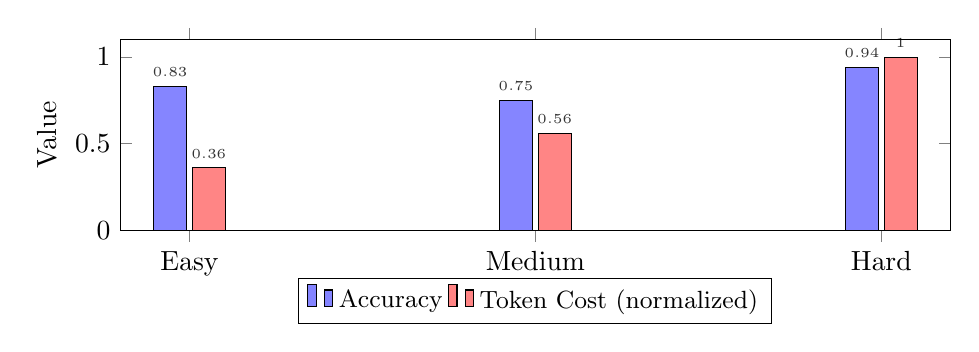
\begin{tikzpicture}
\begin{axis}[
    ybar,
    width=\columnwidth,
    height=4cm,
    bar width=12pt,
    ylabel={Value},
    symbolic x coords={Easy,Medium,Hard},
    xtick=data,
    ymin=0,ymax=1.1,
    legend style={at={(0.5,-0.25)},anchor=north,legend columns=2,font=\small},
    nodes near coords,
    nodes near coords style={font=\tiny},
    every axis plot/.append style={fill opacity=0.8}
]
\addplot[fill=blue!60] coordinates {(Easy,0.83) (Medium,0.75) (Hard,0.94)};
\addplot[fill=red!60] coordinates {(Easy,0.36) (Medium,0.56) (Hard,1.0)};
\legend{Accuracy, Token Cost (normalized)}
\end{axis}
\end{tikzpicture}

\subsection{Key Findings}

\textbf{Finding 1:} Hard prompts cost 2.8$\times$ more tokens (28K$\to$79K) but maintain 94\% accuracy. Tool output scales 6.9$\times$ (5K$\to$34K chars).

\textbf{Finding 2:} 97.9\% of tokens are input -- context accumulation from tool outputs re-sent each turn. This is the core inefficiency MCP tools address.

\textbf{Finding 3:} Token variance is high -- Prompt~4 scored 1.0 on all trials but ranged 51K--99K tokens (1.9$\times$). Deterministic MCP responses eliminate this.

\subsection{Projected MCP Improvement}

\begin{table}[h]
\centering\small
\begin{tabular}{lccc}
\toprule
\textbf{Metric} & \textbf{Raw CLI} & \textbf{MCP (proj.)} & \textbf{Reduction} \\
\midrule
Tokens/prompt & 49,732 & $\sim$8,000 & $\sim$6$\times$ \\
Tool calls & 3.5 & 1.2 & $\sim$3$\times$ \\
Cost/prompt & \$0.058 & $\sim$\$0.012 & $\sim$5$\times$ \\
\bottomrule
\end{tabular}
\end{table}

\subsection{What Remains}

Experiment~1 MCP arm (Apr 1--7, needs v1). Experiment~2 (Apr 7--9, if time). Experiment~3 (future work). \textbf{Worst case:} descope to Experiment~1 only. \textbf{Base case:} v1 by Apr~5, MCP experiment Apr~6--7, Experiment~2 Apr~8--9, report Apr~10.

\section{Impact}

\textbf{DevOps teams} save $\sim$\$1,679/year per project at 100 queries/day. \textbf{Platform engineers} get deterministic responses instead of hallucinated configs. \textbf{Terraform community} gets an open-source MCP server for any MCP-compliant client. \textbf{Classmates} can install and test with zero cloud charges (\texttt{null\_resource} only). If results confirm 6$\times$ token reduction, the approach generalizes to any domain where LLMs interact with large structured state.

\begin{thebibliography}{10}
\small
\bibitem{mcp} Anthropic, ``Introducing the Model Context Protocol,'' Nov 2024.
\bibitem{spec} Model Context Protocol Specification, 2025.
\bibitem{infoq} S. De Simone, ``Anthropic Publishes MCP Specification,'' InfoQ, Dec 2024.
\bibitem{gorilla} S. Patil et al., ``Gorilla: LLM Connected with Massive APIs,'' arXiv 2023.
\bibitem{bfcl} S. Patil et al., ``Berkeley Function Calling Leaderboard,'' ICML 2025.
\bibitem{toolace} Team-ACE, ``ToolACE: Winning the Points of LLM Function Calling,'' Sep 2024.
\bibitem{tfgraph} HashiCorp, ``Terraform Resource Graph.''
\bibitem{terraformer} P. Jana et al., ``TerraFormer: Automated IaC with LLMs,'' Jan 2026.
\bibitem{lost} N. Liu et al., ``Lost in the Middle,'' TACL 2024.
\bibitem{rot} Chroma Research, ``Context Rot,'' 2025.
\end{thebibliography}

\end{document}
